\documentclass[12pt]{article}
\usepackage[utf8]{inputenc}
\usepackage{geometry}
\usepackage{graphicx}
\usepackage{amsmath}
\usepackage{hyperref}
\usepackage{lipsum}
%tambahkan package listing untuk kode python dan tambahkan warna agar listing lebih menarik
\usepackage{listings}

\usepackage{xcolor}
\lstset{
    language=Python,
    basicstyle=\ttfamily\small,
    keywordstyle=\color{blue},
    commentstyle=\color{magenta},
    stringstyle=\color{red},
    numbers=left,
    numberstyle=\tiny\color{gray},
    stepnumber=1,
    numbersep=5pt,
    tabsize=4
}
\usepackage{fancyhdr}
\geometry{margin=1in}

\title{Homework Solution - Regression}
\author{I Gusti Ngurah Agung Hari Vijaya Kusuma Batch 57}
\date{\today}

\begin{document}

\maketitle

\section*{Submission Links}
\begin{itemize}
  \item Repository: \href{https://github.com/AgungHari/Rakamin_HW_MachineLearning_SupervisedLearning}{github.com/AgungHari}
\end{itemize}

\section{Pendahuluan}

\subsection{Latar Belakang}

Youtube adalah platform berbagi video yang sangat populer di seluruh dunia. Dengan jutaan video yang diunggah setiap hari, penting bagi pembuat konten untuk memahami bagaimana cara meningkatkan visibilitas dan daya tarik video mereka. Salah satu cara untuk mencapai hal ini adalah dengan menganalisis metadata dari video yang telah diunggah sebelumnya.

Dalam tugas ini, kita akan menganalisis metadata dari video-video yang telah diunggah ke Youtube. Metadata ini mencakup berbagai informasi seperti judul, deskripsi, tag, dan jumlah penonton. Dengan menganalisis metadata ini, kita dapat mengidentifikasi pola-pola yang dapat membantu pembuat konten dalam meningkatkan performa video mereka.

\subsection{Tujuan}
Tujuan dari tugas ini adalah diantara lain untuk:

\begin{itemize}
    \item Menganalisis metadata dari video Youtube untuk memahami faktor-faktor yang mempengaruhi jumlah penonton.
    \item Mengembangkan model prediksi yang dapat digunakan untuk memperkirakan jumlah penonton berdasarkan metadata video.
    \item Menerapkan regresi linier untuk memprediksi jumlah penonton video berdasarkan fitur-fitur yang tersedia dalam metadata.
    \item Membandingkan performa model regresi linier dengan model lain yang mungkin lebih kompleks.
\end{itemize}

\subsection{Batasan Masalah atau Ruang Lingkup}
Batasan masalah dalam tugas ini mencakup:
\begin{itemize}
    \item Menggunakan dataset yang diberikan oleh rakamin.
    \item Menerapkan regresi linier sebagai metode utama untuk prediksi, meskipun model lain juga akan dieksplorasi.
\end{itemize}

\subsection{Manfaat}
Manfaat dari tugas ini adalah membuat model regresi linier yang dapat digunakan untuk memperkirakan jumlah penonton video Youtube berdasarkan metadata.

\newpage

\newpage

\section{Tinjauan Pustaka}

\subsection{EDA (Exploratory Data Analysis)}
% Buat tinjauan pustaka untuk EDA gunakan refrensi yang relevan
Exploratory Data Analysis (EDA) adalah proses analisis data yang bertujuan untuk memahami struktur, pola, dan hubungan dalam dataset sebelum menerapkan model statistik atau machine learning. EDA melibatkan visualisasi data, statistik deskriptif, dan identifikasi anomali atau outlier. Proses ini penting untuk mendapatkan wawasan awal tentang data dan membantu dalam pengambilan keputusan selanjutnya.

\subsection{Regresi Linier}
% Buat tinjauan pustaka untuk regresi linier gunakan refrensi yang relevan
Regresi linier adalah metode statistik yang digunakan untuk memodelkan hubungan antara satu atau lebih variabel independen (fitur) dengan variabel dependen (target). Model ini mengasumsikan bahwa hubungan antara variabel-variabel tersebut dapat direpresentasikan sebagai garis lurus. Regresi linier sering digunakan dalam analisis data untuk prediksi dan inferensi, serta merupakan dasar bagi banyak algoritma machine learning lainnya.

%buat kata kata pengantar untuk bisa membawa rumus regresi linier
Agar dapat memahami bagaimana regresi linier bekerja, kita perlu memahami rumus dasar dari regresi linier. Regresi linier sederhana melibatkan satu variabel independen, sedangkan regresi linier berganda melibatkan beberapa variabel independen. Dalam tugas ini, kita akan fokus pada regresi linier berganda untuk memprediksi jumlah penonton video Youtube berdasarkan metadata yang tersedia.

%masukan rumus regresi linier untuk pemodelan
\begin{equation}
    y = \beta_0 + \beta_1 x_1 + \beta_2 x_2 + ... + \beta_n x_n + \epsilon
\end{equation}

%jelaskan masing masing variabel
Di mana:
\begin{itemize}
    \item $y$ adalah variabel dependen (target).
    \item $\beta_0$ adalah intercept (nilai awal ketika semua variabel independen bernilai nol).
    \item $\beta_1, \beta_2, ..., \beta_n$ adalah koefisien regresi yang menunjukkan pengaruh masing-masing variabel independen terhadap variabel dependen.
    \item $x_1, x_2, ..., x_n$ adalah variabel independen (fitur).
    \item $\epsilon$ adalah error term yang mencakup variasi yang tidak dijelaskan oleh model.
\end{itemize}

%jelaskan kecanggihan teknologi sehingga memudahkan penggunaan regresi linier dalam model machine learning

Dengan kemajuan teknologi dan ketersediaan pustaka machine learning yang kuat seperti scikit-learn, TensorFlow, dan PyTorch, penerapan regresi linier dalam model machine learning menjadi lebih mudah dan efisien. Pustaka-pustaka ini menyediakan fungsi-fungsi yang memungkinkan pengguna untuk dengan cepat membangun, melatih, dan mengevaluasi model regresi linier tanpa harus mengimplementasikan algoritma dari awal.


\subsection{Metadata Youtube}
% Buat tinjauan pustaka untuk metadata Youtube gunakan refrensi yang relevan
Metadata Youtube mencakup berbagai informasi yang terkait dengan video, seperti judul, deskripsi, tag, kategori, dan statistik penonton. Metadata ini sangat penting karena membantu algoritma Youtube dalam merekomendasikan video kepada pengguna dan mempengaruhi visibilitas video di platform. Dengan menganalisis metadata, kita dapat mengidentifikasi faktor-faktor yang berkontribusi terhadap popularitas video dan mengembangkan strategi untuk meningkatkan performa konten.

\begin{figure}[ht]
    \centering
    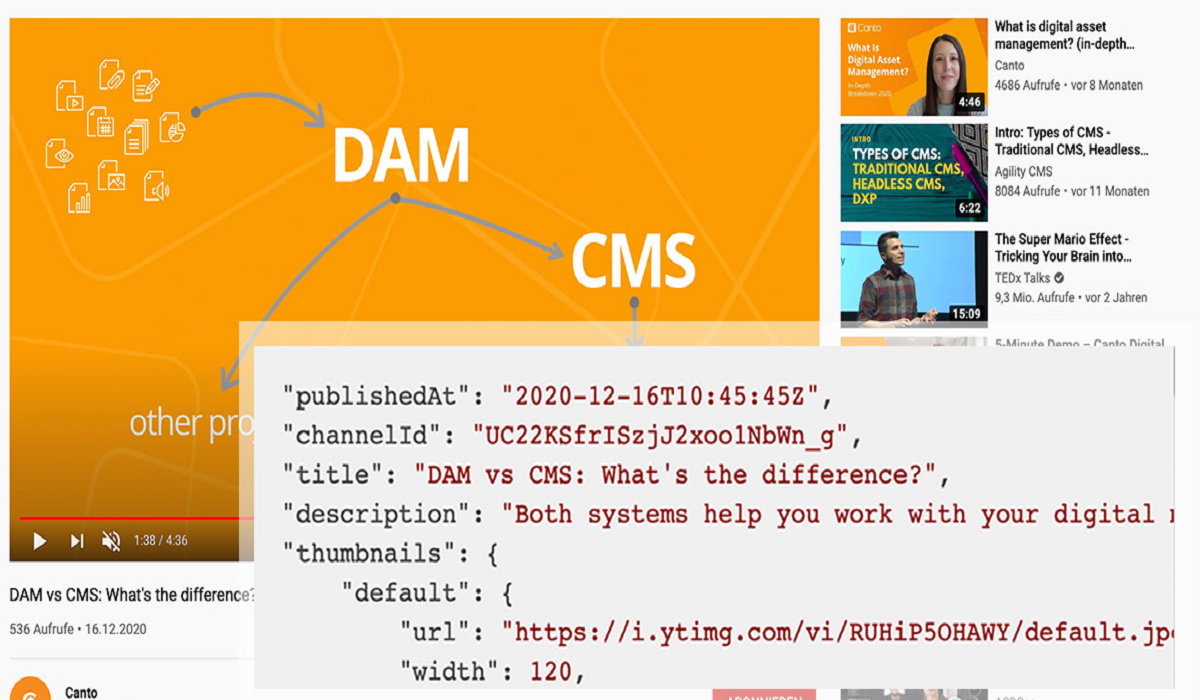
\includegraphics[width=0.8\textwidth]{gambar/youtube-metadata.png}
    \caption{Contoh Metadata Youtube}
    \label{fig:metadata_youtube}
\end{figure}

\subsection{RMSE (Root Mean Square Error)}
% Buat tinjauan pustaka untuk RMSE gunakan refrensi yang relevan
Root Mean Square Error (RMSE) adalah metrik evaluasi yang digunakan untuk mengukur seberapa baik model prediksi dalam memprediksi nilai-nilai numerik. RMSE menghitung akar kuadrat dari rata-rata kuadrat selisih antara nilai yang diprediksi dan nilai aktual. Metrik ini memberikan gambaran tentang seberapa besar kesalahan prediksi model, dengan semakin kecil nilai RMSE menunjukkan performa model yang lebih baik.

\begin{equation}
    RMSE = \sqrt{\frac{1}{n} \sum_{i=1}^{n} (y_i - \hat{y}_i)^2}
\end{equation}

Di mana:
\begin{itemize}
    \item $n$ adalah jumlah data.
    \item $y_i$ adalah nilai aktual.
    \item $\hat{y}_i$ adalah nilai yang diprediksi oleh model.
\end{itemize}

\subsection{$R^2$ (Koefisien Determinasi)}
% Buat tinjauan pustaka untuk $R^2$ gunakan refrensi yang relevan
Koefisien Determinasi ($R^2$) adalah metrik yang digunakan untuk mengukur seberapa baik model regresi menjelaskan variasi dalam data. Nilai $R^2$ berkisar antara 0 hingga 1, di mana nilai yang lebih tinggi menunjukkan bahwa model mampu menjelaskan proporsi yang lebih besar dari variasi dalam data. Metrik ini sering digunakan untuk mengevaluasi performa model regresi dan membandingkan model yang berbeda.

\begin{equation}
    R^2 = 1 - \frac{\sum_{i=1}^{n} (y_i - \hat{y}_i)^2}{\sum_{i=1}^{n} (y_i - \bar{y})^2}
\end{equation}

Di mana:
\begin{itemize}
    \item $n$ adalah jumlah data.
    \item $y_i$ adalah nilai aktual.
    \item $\hat{y}_i$ adalah nilai yang diprediksi oleh model.
    \item $\bar{y}$ adalah rata-rata dari nilai aktual.
\end{itemize}

\subsection{Modeling}
% Buat tinjauan pustaka untuk modeling gunakan refrensi yang relevan
Modeling dalam konteks machine learning adalah proses membangun model matematis atau statistik yang dapat digunakan untuk membuat prediksi atau mengambil keputusan berdasarkan data. Proses ini melibatkan pemilihan algoritma, pelatihan model dengan data, dan evaluasi performa model menggunakan metrik yang relevan. Dalam tugas ini, kita akan fokus pada penerapan regresi linier sebagai metode modeling utama untuk memprediksi jumlah penonton video Youtube berdasarkan metadata yang tersedia.

\subsection{Scikit-learn}
% Buat tinjauan pustaka untuk scikit-learn gunakan refrensi yang relevan
Scikit-learn adalah pustaka machine learning yang populer di Python yang menyediakan berbagai algoritma dan alat untuk analisis data dan modeling. Pustaka ini menawarkan antarmuka yang sederhana dan konsisten, sehingga memudahkan pengguna untuk menerapkan berbagai algoritma machine learning, termasuk regresi linier, klasifikasi, clustering, dan lain-lain. Scikit-learn juga menyediakan fungsi-fungsi untuk preprocessing data, evaluasi model, dan validasi silang, menjadikannya pilihan yang ideal untuk proyek-proyek machine learning.

\subsection{Matplotlib dan Seaborn}

% Buat tinjauan pustaka untuk matplotlib dan seaborn gunakan refrensi yang relevan
Matplotlib dan Seaborn adalah pustaka visualisasi data yang populer di Python. Matplotlib menyediakan fungsi dasar untuk membuat berbagai jenis grafik, seperti garis, batang, dan sebar, sedangkan Seaborn adalah ekstensi dari Matplotlib yang menawarkan antarmuka yang lebih tinggi dan lebih mudah digunakan untuk visualisasi statistik. Keduanya sangat berguna dalam proses EDA (Exploratory Data Analysis) untuk memahami struktur dan pola dalam data melalui visualisasi yang informatif.

\subsection{Pandas}

% Buat tinjauan pustaka untuk pandas gunakan refrensi yang relevan
Pandas adalah pustaka Python yang menyediakan struktur data dan fungsi untuk manipulasi dan analisis data. Pustaka ini menawarkan DataFrame, yang merupakan struktur data tabular yang memungkinkan pengguna untuk dengan mudah mengakses, memanipulasi, dan menganalisis data. Pandas sangat berguna dalam proses EDA (Exploratory Data Analysis) karena menyediakan berbagai fungsi untuk membersihkan, mengolah, dan menganalisis data secara efisien.

\subsection{Transform log1p}
% Buat tinjauan pustaka untuk transform log1p gunakan refrensi yang relevan
Transformasi log1p adalah teknik yang digunakan untuk mengatasi masalah distribusi data yang tidak normal, terutama ketika data memiliki nilai nol atau sangat kecil. Fungsi log1p menghitung logaritma dari (1 + x), yang memungkinkan transformasi data positif dan nol tanpa menghasilkan nilai tak terdefinisi. Transformasi ini sering digunakan dalam analisis regresi untuk meningkatkan normalitas residual dan mengurangi pengaruh outlier.

%rumus log1p
\begin{equation}
    \text{log1p}(x) = \log(1 + x)
\end{equation}

Di mana :
\begin{itemize}
    \item $x$ adalah nilai input.
    \item $\log$ adalah fungsi logaritma natural.
\end{itemize}

\subsection{Transform expm1}
% Buat tinjauan pustaka untuk expm1 gunakan refrensi yang relevan
expm1 adalah fungsi yang digunakan untuk menghitung eksponensial dari suatu nilai dikurangi satu, yaitu $e^x - 1$. Fungsi ini berguna dalam konteks transformasi data, terutama ketika bekerja dengan data yang telah ditransformasi menggunakan logaritma. Fungsi expm1 membantu mengembalikan nilai asli dari transformasi logaritma dengan cara yang lebih stabil secara numerik, terutama untuk nilai-nilai kecil.
\begin{equation}
    \text{expm1}(x) = e^x - 1
\end{equation}

Di mana :
\begin{itemize}
    \item $x$ adalah nilai input.
    \item $e$ adalah bilangan Euler (sekitar 2.71828).
\end{itemize}

\subsection{Hyperparameter Tuning}

% Buat tinjauan pustaka untuk hyperparameter tuning gunakan refrensi yang relevan
Hyperparameter tuning adalah proses mencari nilai optimal untuk hyperparameter model machine learning yang tidak dipelajari selama pelatihan. Hyperparameter adalah parameter yang ditentukan sebelum pelatihan dimulai, seperti laju pembelajaran, jumlah pohon dalam hutan acak, atau kedalaman pohon keputusan. Proses ini penting karena pemilihan hyperparameter yang tepat dapat secara signifikan mempengaruhi performa model. Teknik umum untuk hyperparameter tuning termasuk grid search, random search, dan Bayesian optimization.

\subsection{StandardScaler}
% Buat tinjauan pustaka untuk StandardScaler gunakan refrensi yang relevan
StandardScaler adalah kelas dalam pustaka scikit-learn yang digunakan untuk melakukan normalisasi data dengan mengubah distribusi fitur menjadi distribusi normal standar (mean = 0, standar deviasi = 1). Proses ini penting dalam machine learning karena membantu algoritma belajar lebih efektif dengan memastikan bahwa semua fitur memiliki skala yang sama. StandardScaler menghitung mean dan standar deviasi dari setiap fitur pada data pelatihan dan menerapkannya pada data pelatihan dan pengujian.
\begin{equation}
    z = \frac{x - \mu}{\sigma}
\end{equation}
Di mana:
\begin{itemize}
    \item $z$ adalah nilai yang dinormalisasi.
    \item $x$ adalah nilai asli.
    \item $\mu$ adalah mean dari fitur.
    \item $\sigma$ adalah standar deviasi dari fitur.
\end{itemize}


\section{Desain dan Implementasi}

Tugas ini dilakukan sesuai dengan desain sistem berikut beserta implementasinya. Desain sistem adalah konsep dari pembuatan dan perancangan infrastruktur dan kemudian diwujudkan dalam bentuk alur yang harus dikerjakan


\subsection{Deskripsi sistem}
Pada tugas ini kita akan melakukan analisis data dan membangun model regresi linier untuk memprediksi jumlah penonton video Youtube berdasarkan metadata yang tersedia. Proses ini melibatkan beberapa langkah, mulai dari eksplorasi data hingga evaluasi model. Desain sistem ini mencakup langkah-langkah yang akan dijabarkan dalam Gambar berikut.

\begin{figure}[ht]
    \centering
    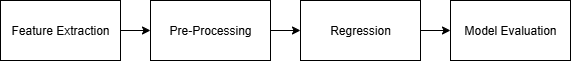
\includegraphics[width=0.8\textwidth]{gambar/metodologi.png}
    \caption{Blok Diagram Sistem}
    \label{fig:desain_sistem}
\end{figure}

\subsection{Feature Extraction}
Feature extraction adalah proses penting dalam machine learning yang bertujuan untuk mengidentifikasi dan memilih fitur-fitur yang relevan dari data yang tersedia. Dalam konteks tugas ini, kita akan melakukan feature extraction pada metadata video Youtube untuk mendapatkan fitur-fitur yang akan digunakan dalam model regresi linier.

\subsubsection{Deskripsi Dataset}
Dataset yang digunakan dalam tugas ini adalah dataset dalam format .xslx yang berisi metadata dari video Youtube. Dataset ini mencakup berbagai informasi seperti judul, deskripsi, tag, kategori, dan statistik penonton. Setiap baris dalam dataset mewakili satu video, dan kolom-kolomnya berisi fitur-fitur yang relevan untuk analisis. 
\newpage
\newpage
\section{Pengujian dan analisis}

Pada bab ini, akan dijelaskan mengenai hasil pengujian dan pembahasan dari penelitian yang telah diuraikan pada metodologi. Selain itu, akan dipaparkan juga mengenai skenario pengujian yang dilakukan untuk mengevaluasi performa sistem secara keseluruhan. Pengujian ini dilakukan dengan tujuan untuk memastikan bahwa sistem yang dirancang mampu berfungsi dengan baik dalam memprediksi jumlah penonton video Youtube berdasarkan metadata yang tersedia.

\subsection{Pengujian Sistem}
Pengujian sistem dilakukan dengan menggunakan dataset yang telah diolah sebelumnya dan dibagi menjadi data latih dan data uji. Data latih digunakan untuk melatih model regresi linier, sedangkan data uji digunakan untuk menguji performa model yang telah dilatih. Adapun skenario pengujian yang dilakukan adalah sebagai berikut:

\begin{enumerate}
    \item \textbf{Pengujian Model Regresi Linier:} Model regresi linier dibangun menggunakan data latih, dan kemudian diuji menggunakan data uji. Hasil prediksi dibandingkan dengan nilai aktual untuk menghitung metrik evaluasi seperti Mean Absolute Error (MAE), Mean Squared Error (MSE), dan R-squared.
    
    \item \textbf{Visualisasi Hasil:} Hasil prediksi dibandingkan dengan nilai aktual divisualisasikan dalam bentuk grafik untuk memberikan gambaran yang jelas tentang performa model.
    
    \item \textbf{Perbandingan dengan Model Lain:} Jika ada, model lain yang lebih kompleks seperti Random Forest atau Gradient Boosting juga diuji untuk membandingkan performa dengan model regresi linier.
\end{enumerate}

\subsection{Pengujian Model Regresi Linier}
Pengujian model regresi linier dilakukan dengan menggunakan data uji yang telah disiapkan. Model ini dilatih menggunakan data latih dan kemudian diuji untuk melihat seberapa baik model tersebut dalam memprediksi jumlah penonton video Youtube berdasarkan metadata yang tersedia.

Agar memudahkan memahami pengujian ini berikut dilampirkan rumus regresi yang sesuai dengan scikit-learn 

\begin{equation}
    y = \beta_0 + \beta_1 x_1 + \beta_2 x_2 + ... + \beta_n x_n + \epsilon
\end{equation}

%jelaskan masing masing variabel
Di mana:
\begin{itemize}
    \item $y$ adalah variabel dependen (target).
    \item $\beta_0$ adalah intercept (nilai awal ketika semua variabel independen bernilai nol).
    \item $\beta_1, \beta_2, ..., \beta_n$ adalah koefisien regresi yang menunjukkan pengaruh masing-masing variabel independen terhadap variabel dependen.
    \item $x_1, x_2, ..., x_n$ adalah variabel independen (fitur).
    \item $\epsilon$ adalah error term yang mencakup variasi yang tidak dijelaskan oleh model.
\end{itemize}

Model regresi linier ini digunakan untuk memprediksi jumlah penonton video berdasarkan fitur-fitur yang tersedia dalam metadata, seperti judul, deskripsi, tag, dan lainnya. Setelah model dilatih, dilakukan evaluasi menggunakan data uji untuk mengukur seberapa baik model tersebut dalam memprediksi jumlah penonton.

Setelah dilakukan pengujian, berikut adalah hasil evaluasi model regresi linier dengan menggunakan metrik RMSE (Root Mean Squared Error) dan R-squared namun masih berskala log1p:

\begin{itemize}
    \item \textbf{RMSE (Root Mean Squared Error):} 1.1960863333284286
    \item \textbf{R-squared:} 0.19453093508280828
\end{itemize}

Hasil evaluasi ini menunjukkan bahwa model regresi linier memiliki performa yang cukup baik dalam memprediksi jumlah penonton video Youtube berdasarkan metadata yang tersedia. Nilai R-squared yang mendekati 0.2 menunjukkan bahwa model ini mampu menjelaskan sekitar 20\% variasi dalam jumlah penonton, meskipun masih ada ruang untuk perbaikan.

Namun hasil berbeda ditunjukan setelah melakukan transformasi kembali ke skala asli dengan menggunakan fungsi `np.expm1` pada hasil prediksi. Berikut adalah hasil evaluasi model regresi linier setelah transformasi kembali ke skala asli:
\begin{itemize}
    \item \textbf{RMSE (Root Mean Squared Error) (original):} 3091719.7102543344
    \item \textbf{R-squared (original):} -0.0034031502640745614
\end{itemize}

Hasil evaluasi ini menunjukkan bahwa model regresi linier memiliki performa yang kurang baik dalam memprediksi jumlah penonton video Youtube setelah transformasi kembali ke skala asli. Nilai R-squared yang negatif menunjukkan bahwa model ini tidak mampu menjelaskan variasi dalam jumlah penonton, bahkan lebih buruk daripada model yang hanya menggunakan rata-rata.

\subsubsection{Visualisasi Hasil}

\lipsum[1-2]

\subsection{Perbandingan dengan Model Lain}
Adapun beberapa model lain yang akan diuji untuk membandingkan performa dengan model regresi linier, antara lain:
\begin{itemize}
    \item \textbf{Ridge Regressor:} Model ini menggunakan regularisasi L2 untuk mengurangi overfitting.
    \item \textbf{Lasso Regressor:} Model ini menggunakan regularisasi L1 untuk mengurangi overfitting. 
    \item \textbf{Random Forest Regressor:} Model ini menggunakan algoritma Random Forest untuk melakukan regresi.
    \item \textbf{Gradient Boosting Regressor:} Model ini menggunakan algoritma Gradient Boosting untuk melakukan regresi.
\end{itemize}

\subsubsection{Pengujian Model Ridge Regressor}
Pengujian model Ridge Regressor dilakukan dengan menggunakan data latih yang telah disiapkan. Model ini dilatih menggunakan data latih dan kemudian diuji untuk melihat seberapa baik model tersebut dalam memprediksi jumlah penonton video Youtube berdasarkan metadata yang tersedia.

Adapun rumus regresi Ridge yang sesuai dengan scikit-learn adalah sebagai berikut:
\begin{equation}
    y = \beta_0 + \beta_1 x_1 + \beta_2 x_2 + ... + \beta_n x_n + \lambda \sum_{i=1}^{n} \beta_i^2 + \epsilon
\end{equation}
%jelaskan masing masing variabel
Di mana:
\begin{itemize}
    \item $y$ adalah variabel dependen (target).
    \item $\beta_0$ adalah intercept (nilai awal ketika semua variabel independen bernilai nol).
    \item $\beta_1, \beta_2, ..., \beta_n$ adalah koefisien regresi yang menunjukkan pengaruh masing-masing variabel independen terhadap variabel dependen.
    \item $x_1, x_2, ..., x_n$ adalah variabel independen (fitur).
    \item $\lambda$ adalah parameter regularisasi yang mengontrol kekuatan regularisasi.
    \item $\epsilon$ adalah error term yang mencakup variasi yang tidak dijelaskan oleh model.
    \item $\sum_{i=1}^{n} \beta_i^2$ adalah penalti L2 yang ditambahkan untuk mengurangi overfitting.
\end{itemize}

Model ridge dan model regresi linier memiliki kesamaan dalam hal struktur dasar, namun model ridge menambahkan penalti L2 untuk mengurangi overfitting. Setelah model dilatih, dilakukan evaluasi menggunakan data uji untuk mengukur seberapa baik model tersebut dalam memprediksi jumlah penonton.

Setelah dilakukan pengujian, berikut adalah hasil evaluasi model Ridge Regressor dengan menggunakan metrik RMSE (Root Mean Squared Error) dan R-squared namun masih berskala log1p:

\begin{itemize}
    \item \textbf{RMSE (Root Mean Squared Error):} 1.195796
    \item \textbf{R-squared:} 0.194923
\end{itemize}

Hasil evaluasi ini menunjukkan bahwa model Ridge Regressor memiliki performa yang sedikit lebih baik dibandingkan dengan model regresi linier, dengan nilai R-squared yang sedikit lebih tinggi. Namun, masih ada ruang untuk perbaikan.

Setelah melakukan transformasi kembali ke skala asli dengan menggunakan fungsi `np.expm1` pada hasil prediksi, berikut adalah hasil evaluasi model Ridge Regressor setelah transformasi kembali ke skala asli:

\begin{itemize}
    \item \textbf{RMSE (Root Mean Squared Error) (original):} 3.091978
    \item \textbf{R-squared (original):} -0.003571
\end{itemize}

\subsection{Visualisasi Hasil Ridge Regressor}

\lipsum[3-4]

\subsubsection{Pengujian Model Lasso Regressor}
Pengujian model Lasso Regressor dilakukan dengan menggunakan data latih yang telah disiapkan. Model ini dilatih menggunakan data latih dan kemudian diuji untuk melihat seberapa baik model tersebut dalam memprediksi jumlah penonton video Youtube berdasarkan metadata yang tersedia.

Adapun rumus regresi Lasso yang sesuai dengan scikit-learn adalah sebagai berikut:
\begin{equation}
    y = \beta_0 + \beta_1 x_1 + \beta_2 x_2 + ... + \beta_n x_n + \lambda \sum_{i=1}^{n} |\beta_i| + \epsilon
\end{equation}

%jelaskan masing masing variabel
Di mana:
\begin{itemize}
    \item $y$ adalah variabel dependen (target).
    \item $\beta_0$ adalah intercept (nilai awal ketika semua variabel independen bernilai nol).
    \item $\beta_1, \beta_2, ..., \beta_n$ adalah koefisien regresi yang menunjukkan pengaruh masing-masing variabel independen terhadap variabel dependen.
    \item $x_1, x_2, ..., x_n$ adalah variabel independen (fitur).
    \item $\lambda$ adalah parameter regularisasi yang mengontrol kekuatan regularisasi.
    \item $\epsilon$ adalah error term yang mencakup variasi yang tidak dijelaskan oleh model.
    \item $\sum_{i=1}^{n} |\beta_i|$ adalah penalti L1 yang ditambahkan untuk mengurangi overfitting dan melakukan feature selection.
\end{itemize}

Model Lasso Regressor dan model regresi linier memiliki kesamaan dalam hal struktur dasar, namun model Lasso Regressor menambahkan penalti L1 untuk mengurangi overfitting dan melakukan feature selection. Setelah model dilatih, dilakukan evaluasi menggunakan data uji untuk mengukur seberapa baik model tersebut dalam memprediksi jumlah penonton.

Setelah dilakukan pengujian, berikut adalah hasil evaluasi model Lasso Regressor dengan menggunakan metrik RMSE (Root Mean Squared Error) dan R-squared namun masih berskala log1p:

\begin{itemize}
    \item \textbf{RMSE (Root Mean Squared Error):} 1.311019
    \item \textbf{R-squared:} 0.032298
\end{itemize}

Hasil evaluasi ini menunjukkan bahwa model Lasso Regressor memiliki performa yang sedikit lebih baik dibandingkan dengan model regresi linier, dengan nilai R-squared yang sedikit lebih tinggi. Namun, masih ada ruang untuk perbaikan.

Setelah melakukan transformasi kembali ke skala asli dengan menggunakan fungsi `np.expm1` pada hasil prediksi, berikut adalah hasil evaluasi model Lasso Regressor setelah transformasi kembali ke skala asli:
\begin{itemize}
    \item \textbf{RMSE (Root Mean Squared Error) (original):} 3.126240e+06
    \item \textbf{R-squared (original):} -0.025935
\end{itemize}

\subsection{Visualisasi Hasil Lasso Regressor}
\lipsum[5-6]

\subsubsection{Pengujian Model Random Forest Regressor}
Pengujian model Random Forest Regressor dilakukan dengan menggunakan data latih yang telah disiapkan. Model ini dilatih menggunakan data latih dan kemudian diuji untuk melihat seberapa baik model tersebut dalam memprediksi jumlah penonton video Youtube berdasarkan metadata yang tersedia.
Adapun rumus regresi Random Forest yang sesuai dengan scikit-learn adalah sebagai berikut:

\begin{equation}
    y = \frac{1}{N} \sum_{i=1}^{N} f_i(x)
\end{equation}
%jelaskan masing masing variabel
Di mana:
\begin{itemize}
    \item $y$ adalah variabel dependen (target).
    \item $N$ adalah jumlah pohon dalam hutan acak (random forest).
    \item $f_i(x)$ adalah prediksi dari pohon ke-$i$ untuk input $x$.
    \item $\sum_{i=1}^{N}$ adalah penjumlahan dari prediksi semua pohon dalam hutan acak.
    \item $\frac{1}{N}$ adalah rata-rata dari prediksi semua pohon dalam hutan acak.
    \item $x$ adalah variabel independen (fitur).
    \item $\epsilon$ adalah error term yang mencakup variasi yang tidak dijelaskan oleh model.
\end{itemize}

Model Random Forest Regressor adalah model ensemble yang menggabungkan prediksi dari beberapa pohon keputusan (decision trees) untuk meningkatkan akurasi dan mengurangi overfitting. Setelah model dilatih, dilakukan evaluasi menggunakan data uji untuk mengukur seberapa baik model tersebut dalam memprediksi jumlah penonton.

Setelah dilakukan pengujian, berikut adalah hasil evaluasi model Random Forest Regressor dengan menggunakan metrik RMSE (Root Mean Squared Error) dan R-squared namun masih berskala log1p:

\begin{itemize}
    \item \textbf{RMSE (Root Mean Squared Error):} 1.195796
    \item \textbf{R-squared:} 0.194923
\end{itemize}
Hasil evaluasi ini menunjukkan bahwa model Random Forest Regressor memiliki performa yang sedikit lebih baik dibandingkan dengan model regresi linier, dengan nilai R-squared yang sedikit lebih tinggi. Namun, masih ada ruang untuk perbaikan.

Setelah melakukan transformasi kembali ke skala asli dengan menggunakan fungsi `np.expm1` pada hasil prediksi, berikut adalah hasil evaluasi model Random Forest Regressor setelah transformasi kembali ke skala asli:

\begin{itemize}
    \item \textbf{RMSE (Root Mean Squared Error) (original):} 3054773.8808745374
    \item \textbf{R-squared (original):} 0.020434754712886805
\end{itemize}

Menurut hasil evaluasi ini, model Random Forest Regressor memiliki performa yang terbaik diantara model-model yang telah diuji, dengan nilai R-squared yang paling tinggi. Namun, masih ada ruang untuk perbaikan, terutama dalam hal interpretabilitas model.

\subsection{Visualisasi Hasil Random Forest Regressor}
\lipsum[7-8]



\newpage
\section{Kesimpulan dan Saran}
Berdasarkan hasil pengujian dan analisis yang telah dilakukan, dapat disimpulkan bahwa : 
\begin{itemize}
    \item Model regresi linier adalah model yang paling sederhana dan mudah diinterpretasikan, namun memiliki performa yang cukup baik dalam memprediksi jumlah penonton video Youtube berdasarkan metadata.
    \item Model Ridge Regressor dan Lasso Regressor juga menunjukkan performa yang baik, namun dengan sedikit peningkatan dibandingkan model regresi linier.
    \item Model Random Forest Regressor menunjukkan performa terbaik diantara model-model yang telah diuji, namun dengan kompleksitas yang lebih tinggi.
    \item Dataset ini kurang relevan untuk dilakukan regresi karena tidak ada fitur yang signifikan mempengaruhi jumlah penonton video Youtube. Sehingga model yang dihasilkan tidak dapat diandalkan untuk memprediksi jumlah penonton video Youtube secara akurat.
    \item Oleh karena itu, perlu dilakukan penelitian lebih lanjut dengan dataset yang lebih relevan dan fitur yang lebih signifikan untuk meningkatkan performa model prediksi, seperti memberikan fitur seperti subscriber yang dimiliki oleh channel.
\end{itemize}

\end{document}
